\chapter{Noise in optical measurements}

%本章では、光計測における光の検出法について述べるとともに、光計測において生じる雑音について現象論的に説明する。いくつかの説明は天下りであるが、それらは、後の章で量子光学を用いて説明することとする。

\section{Various methods of optical measurement}
\label{section:noise_in_optical_measurement}


%図\ref{fig:photodetection}(a)のように光を光検出器に入射する状況を考えよう。光検出器は光子を電子に変換するデバイスであり、光パワー\footnote{光パワーは単位時間あたりの光エネルギーであるから、光子1個のエネルギーと単位時間あたりのフォトン数の積に等しい。}を計測することができる。これを\textbf{直接検出}\index{ちょくせつけんしゅつ@直接検出}、もしくは\textbf{光子数検出}という。

%また、図\ref{fig:photodetection}(b)のように、計測したい光と別の光(局発光、local oscillator (LO))をビームスプリッタによって\textbf{干渉}させ、出力の光をそれぞれ2つの検出器で計測すると、光の振幅を計測することができる。このことを\textbf{干渉検出}\index{かんしょうけんしゅつ@干渉検出}という。なお、2つの光の周波数が同じ場合は\textbf{ホモダイン検出}\index{ほもだいんけんしゅつ@ホモダイン検出}、周波数が異なる場合を\textbf{ヘテロダイン検出}\index{へてろだいんけんしゅつ@ヘテロダイン検出}という。

%さらに、図\ref{fig:photodetection}(c)のように、光検出の前に光増幅器を用いて光を増幅してから計測する場合もある。このように光検出の直前に光増幅を行うことを光前置増幅という。図\ref{fig:photodetection}には示していないが、光前置増幅を行なった上で干渉検出を行う場合もある。

%いずれの場合も、様々な要因によって信号には雑音が現れる。光源や光学系が不安定であればそれはそのまま雑音となるし、光源や検出器の電子回路も検出時の雑音源となりうる。それらを低減して行った先に最後に必ず残り、姿を現すのが量子雑音である。

%ここでは、雑音について説明する前に、直接検出、干渉検出、光増幅の様子を簡単にまとめておこう。

\begin{figure}
  \centering
  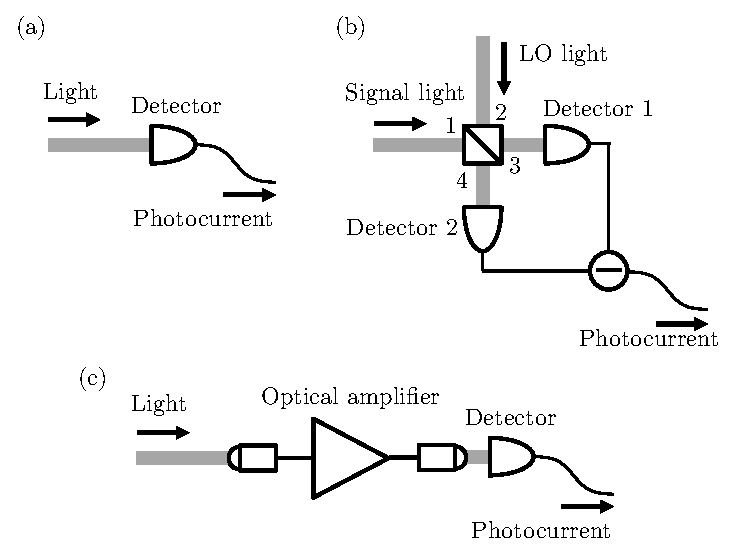
\includegraphics[width=9cm]{fig/1-1_photodetection.eps}
%  \caption{代表的な光検出法。(a) 直接検出。(b) 干渉検出。(c) 光前置増幅。光を光ファイバ増幅器に入力し、光増幅後に直接検出する状況を記載している。}
  \label{fig:photodetection}
\end{figure}

\begin{comment}
\subsection{直接検出}
まず、直接検出における電流と光パワーの関係を求めよう。光パワーを$P$、光子エネルギーを$\hbar \omega$とすると、単位時間あたりに到来する光子数は$P/\hbar \omega$である。入射した光子のうち電子に変換される割合を量子効率といい、$\eta$で表すと、単位時間あたりに発生する伝導電子の数は$\eta P/\hbar \omega$個である。したがって、電荷素量を$q = 1.602 \times 10^{-19} \ \mathrm{[C]}$とすれば、検出器の出力電流は次式で与えられる。
\begin{equation}
	I = \frac{\eta q P}{\hbar \omega}
	\nonumber
\end{equation}
ここで、$I/P = \eta q / \hbar \omega$は\textbf{光電変換効率}\index{こうでんへんかんこうりつ@光電変換効率}と呼ばれる。$\hbar \omega / q$は光子エネルギーをeVで表した値である。光通信波長である1.55 \ \textmu m では光子エネルギーは約0.8 eVである。また、典型的なフォトダイオードの量子効率は90\%程度であるから、この波長帯における光電変換効率は1.1 A/W程度である\footnote{1.5 \ \textmu m帯の光検出に用いられるInGaAsフォトダイオードのカタログを見てみると良い。Googleで``InGaAs pd''というキーワードで検索するといくつか見つかる。}。すなわち、1 mWの光を入力すると約1.1 mAの光電流が得られる。

ひとつの光子が入射した時に、多数の伝導電子が発生するタイプの検出器もあり、なだれフォトダイオード、光電子増倍管などが知られている\footnote{電子の増倍作用を用いたイメージセンサとして、EM-CCD (electron multiplying charge coupled device)も最近登場し、微弱光のイメージングに使われる。}。これは電子の増倍作用を用いて電流信号を大きくすることで検出器そのものの雑音の影響を相対的に小さく抑えることができるため、微弱光の検出に使われる\footnote{これらは増倍のプロセスが確率的であるため、信号対雑音比が3 dB程度低下する。}。

\subsection{干渉検出}

図\ref{fig:photodetection}(b)は典型的な干渉検出の模式図である。信号光と局発光をビームスプリッタで重ね合わせ、ビームスプリッタの2つの出力をそれぞれ別のフォトダイオードで検出する。これらのフォトダイオードが出力する光電流の差分を取る。この測定法を\textbf{バランスド検出法}という。信号光と局発光の周波数をそれぞれ$\omega + \Delta \omega, \omega$とするとき、$\Delta \omega = 0$の場合を\textbf{ホモダイン検出}、$\Delta \omega \neq 0$の場合を\textbf{ヘテロダイン検出}という\footnote{これらの言葉は、電気回路においてミキサを用いて周波数変換を行う場合と対応している。}。

バランスド検出法における出力信号は以下のように求めることができる。信号光と局発光の複素振幅をそれぞれ$\alpha, \beta$としよう。ただし、$|\alpha|^2, |\beta|^2$がそれぞれ時間$\tau$あたりの光子数になるように定義する。また、$\Delta \omega \ll \omega$であり、信号光と局発光の光子エネルギーの差は無視できるものとする\footnote{この仮定を置かないと信号光と局発光の電場の足し引きができない。}。この時、信号光と局発光の解析信号\footnote{電界$E(t)$を$E(t)=\mathrm{Re} \ E_0 e^{-i\omega t}$と書くとき、$E_0$を複素振幅といい、$E_0 e^{-i\omega t}$を解析信号という。つまり、解析信号とは、周波数が正の成分のみから構成されていて、その実部を取ると、実信号になるもの。}は
\begin{equation}
\begin{aligned}
	a(t) &= \alpha e^{-i(\omega + \Delta \omega)t}\\
  	b(t) &= \beta e^{-i\omega t}
\end{aligned}\label{eq:complex_amplitude}
\end{equation}
と表せる。ビームスプリッタのポート1および2にそれぞれ信号光および局発光を入力するときの、ポート3, 4から出力される光の解析信号をそれぞれ$a', b'$とすると、
\begin{equation}
\begin{aligned}
  a' &= \frac{1}{\sqrt 2}(a - b)\\
  b' &= \frac{1}{\sqrt 2}(a + b)
\end{aligned}\label{eq:BS_complex_amplitude}
\end{equation}
と表せる。$a'$の式の右辺で$b$の符号がマイナスになっているのは、ポート2からポート4に固定端反射が生じると仮定したためである\footnote{ポート1から3、もしくはポート2から4のどちらが固定端反射もしくは解放端反射かは、最終的な結果の位相に影響するだけで、全体の結論に大きな影響は及ぼさない。また、後で説明するように、ビームスプリッタを結合導波路として考える場合は、結合する側が$i$倍される。}。式(\ref{eq:BS_complex_amplitude})は行列を用いて
\begin{equation}
  \left( \begin{array}{c}
  	A' \\ B'
  \end{array}
  \right) =
  \frac{1}{\sqrt 2}\left( \begin{array}{r r} 
  	1 & -1 \\ 1 & 1
 \end{array}
	\right)
	\left( \begin{array}{c}
		A \\ B
	\end{array} \right)
	\label{eq:beamsplitter_matrix}
\end{equation}
と書くこともできる\footnote{この行列がユニタリであることは、光パワーの損失がないことに対応している。}。

ポート3, 4から出力される光を検出器1, 2で受光し、その光電流をそれぞれ$I_1, I_2$とすると、
\begin{equation}
\begin{aligned}
  I_1 &= \frac q \tau |a'|^2 = \frac{q}{\tau}\left|\frac{1}{\sqrt 2} (a - b)\right|^2\\
  I_2 &= \frac q \tau |b'|^2 = \frac{q}{\tau}\left|\frac{1}{\sqrt 2} (a + b)\right|^2
\end{aligned}
\end{equation}
を得る。したがって、
\begin{equation}
\begin{aligned}
  I_2 - I_1 &= \frac{q}{\tau}(ab^* + a^* b)\\
  &= 2qB(\alpha \beta^* e^{-i\Delta\omega t} + \alpha^* \beta e^{i\Delta\omega t})\\
  &= 4qB|\beta|\left\{\mathrm{Re} \  (\alpha e^{-i\phi}) \cos \Delta \omega t + \mathrm{Im} \ (\alpha e^{-i\phi}) \sin \Delta \omega t\right\}
\end{aligned}\label{eq:output_of_balanced_detector}
\end{equation}
ただし、$B = 1/2\tau$はナイキスト周波数である。また、$\beta = |\beta|e^{i\phi}$とおいた。

式(\ref{eq:output_of_balanced_detector})より、$\Delta \omega = 0$であれば$I_2 - I_1 = 4qB|\beta| \mathrm{Re} \ (\alpha e^{-i\phi})$であるから、$\alpha$の複素振幅の$\beta$の位相を基準とする軸への射影を計測することが可能であることがわかる。これがホモダイン検出である。

また、$\Delta \omega \neq 0$であれば、光電流には周波数$\Delta \omega$の正弦波が発生することがわかる。この$\cos$成分と$\sin$成分を求めることで、$\alpha$の複素振幅を求めることが可能である。これがヘテロダイン検出である。

\section{光計測における雑音}\label{section:1.2}

ここでは、光計測における基本的な雑音である、ショット雑音と熱雑音についてまとめておこう。また、ホモダインやヘテロダインにおけるショット雑音の影響と、前置増幅を行った場合の雑音についても考えてみよう。熱雑音を回避した場合、信号対雑音比がおよそ光子数のオーダになることが見て取れるであろう。

\subsection{ショット雑音}
まず、天下り的に、光を計測した時に光子が検出器に確率的に到来すると仮定しよう。この時、よく知られているように、光子の個数$k$の分布はポアソン分布に従い、その確率分布は
\begin{equation}
	p(k) = \frac{\lambda^k e^{-\lambda}}{k!}
\end{equation}
で与えられる。ただし、$\lambda$は平均の光子の個数である。

ポアソン分布の特徴として、個数の分散と平均値が等しいことが知られている。このことは、次式によって確かめられる。
\begin{equation}
\begin{aligned}
	V[p(k)] &= \sum_k{(k-\lambda)^2}p(k) = \sum_k{k^2 p(k) - 2\lambda k p(k) + \lambda^2 p(k)} = \sum_k{k^2 p(k) - \lambda^2} \\
	&=\sum_k{k\lambda p(k-1) - \lambda^2} = \lambda\sum_k{\left\{ (k-1)p(k-1) + p(k-1)\right\}}-\lambda^2 = \lambda(\lambda + 1) - \lambda^2 = \lambda
\end{aligned}
\end{equation}
ただし、$\sum_k p(k) = 1$、$\sum_k kp(k) = \lambda$を用いた。

このため、光子数を信号$S$、光子数の標準偏差を雑音$N$とし、信号パワーと雑音パワーの比を信号対雑音比(SNR)とすると、
\begin{equation}
	\mathrm{SNR} = (S/N)^2 = \lambda^2/\lambda = \lambda
\end{equation}
となり、平均の光子数が大きいほどSNRが高くなることがわかる。

このような光子数の揺らぎに由来する光電流の雑音を\textbf{ショット雑音}\index{しょっとざつおん@ショット雑音}という。ショット雑音を電流で表すときは、スペクトル密度で表すことが多い。このために、ある短い時間$\tau$を考え、この時間内に到来する光子数の平均が$\lambda$であるとしよう。このとき$I = q\lambda / \tau$である。ショット雑音の電流を実効値もしくは自乗平均平方根(RMS: root mean square)で表すと、
\begin{equation}
	\begin{aligned}
		I_{\mathrm{shot}} = q\sqrt{\lambda}/\tau = q\sqrt{\frac{I\tau}{q}}/\tau = \sqrt{\frac{qI}{\tau}}
	\end{aligned}
\end{equation}

検出器の帯域を$B$とすると、サンプリング定理より、時間$\tau$ごとに検出する光子数が独立になるためには$B = 1 / 2\tau$の帯域が必要であるから、ショット雑音による電流雑音の実効値は次式で与えられる。
\begin{equation}
	\begin{aligned}
		I_\mathrm{shot}=\sqrt{2qIB}
	\end{aligned}
\end{equation}
なお、$I_\mathrm{shot}$の単位は$\mathrm{[A]}$である。

また、式(\ref{eq:complex_amplitude})と同様の定義を用い、信号光の複素振幅を$\alpha$としてショット雑音限界のSNRを表すと、次式のようになる。
\begin{equation}
  \mathrm{SNR} = I^2 / I_\mathrm{shot}^2 = I/2qB = 2qB|\alpha |^2/2qB = |\alpha|^2
\end{equation}
ただし、$I=q|\alpha|^2/\tau = 2qB|\alpha|^2$を用いた。$|\alpha|^2$は光子数を表すから、この式はショット雑音限界のSNRが光子数と一致することと対応している。

しかし、$\alpha$は連続量であり、離散的な整数である「光子数」と一致する、ということはどういうことであろうか。また、$\alpha$という複素数の位相は光子とどのように関係するのであろうか。これらの点は古典論の議論では明らかにならない。

\subsection{熱雑音}

図1.2(a)に示すように、光検出の際には光電流$I$を抵抗$R$に流し、抵抗の両端に現れる電圧$R I$を検出する場合が多い。抵抗があると、その両端には、実効値電圧
\begin{equation}
	v_\mathrm{th} = \sqrt{4k_\mathrm{B}TRB}
	\label{eq:Johnson_noise}
\end{equation}
を持つ雑音が発生することが知られている。ただし、$k_B$はボルツマン定数、$T$は抵抗の絶対温度、$B$は回路の帯域である。この雑音を\textbf{ジョンソン雑音}\index{じょんそんざつおん@ジョンソン雑音}、もしくは単に熱雑音という。熱雑音は光計測における信号対雑音比の低下要因となるため、熱雑音が光の雑音よりも小さく抑えられるように注意深く測定系を設計する必要がある。
\begin{figure}
  \centering
  \includegraphics[width=7cm]{fig/1-2_PD_circuit.eps} 
  \caption{(a) 典型的な光検出回路。PDに逆バイアスをかけ、光電流$I$を負荷抵抗$R$に流すことで、負荷抵抗に現れる電圧$RI$を検出する。(b) ジョンソン雑音について考えるための仮想的な回路。}
  \label{fig:photodetector}
\end{figure}

ジョンソン雑音の式(式(\ref{eq:Johnson_noise}))を導出するために、図1.2(b)に示す回路を考えよう。抵抗1 ($R_1$)ともう一つの抵抗2 ($R_2$)を接続し、インピーダンスマッチングするように$R_1 = R_2 = R$とする。抵抗1の熱雑音が作る起電力を$v_{th}$とすると、回路一周の抵抗が$2R$であることから、起電力によって流れる電流は$v_{th}/2R$である。この時、この熱雑音が抵抗2に与えるパワーは$v_{th}^2/2R$となる。同様に、抵抗2から抵抗1にも同じパワーが与えられることで、抵抗1と抵抗2が熱平衡状態を保っている\footnote{抵抗1と抵抗2の温度が違う場合は、電気を介して熱の移動が生じる。}。

熱雑音を時間間隔$\tau$でサンプリングする\footnote{この表現はちょっとラフである。もう少し丁寧に表現すると、以下のようになる:熱雑音由来の電圧雑音に対して$-1/2\tau < f < 1/2\tau$までの周波数制限をかけたと仮定しよう。このとき、時間領域で時間間隔$\tau$ごとに離散的にサンプリングすることで電圧波形の情報を得ることができる。これらひとつひとつのサンプリング点が、雑音波形の自由度に対応し、それらにボルツマンエネルギー$k_B T$が分配される。}と、$B = 1/2\tau$までの情報を捉えることができる。各サンプリング間隔において起電力が行う仕事は$v^2_{th}\tau/2R$であり、これら全ての自由度に対してボルツマンエネルギー$k_BT$が分配されることから、次式が成り立つ。
\begin{equation}
v_\mathrm{th}^2\tau/2R = v_\mathrm{th}^2 / 4RB = k_\mathrm{B}T
\end{equation}
この式から式(\ref{eq:Johnson_noise})を得る。
%\footnote{1モードあたり$k_BT/2$ではなく$k_BT$のエネルギーを持つのは、振動子が位置と運動量の2つの自由度を持つため。}

\subsubsection{熱雑音とショット雑音の大きさの比較}
光検出において熱雑音とショット雑音のどちらが支配的かを意識しておくことは重要である。そのイメージを持つために、熱雑音とショット雑音が等しくなる条件を考えてみよう。この条件は、$RI_\mathrm{shot} = v_\mathrm{th}$と表される。この関係が成り立つときの$I$を$I'$とおくと、
\begin{equation}
	I' = 2\frac{k_\mathrm B T }{qR}
\end{equation}
を得る。$k_\mathrm{B}T/q$はボルツマンエネルギーをeVで表したものであり、室温($T$ = 300 K)において$26 \ \mathrm{meV}$である。

負荷抵抗を$R = 50 \ \Omega$とすれば、$I = 1 \ \mathrm{[mA]}$の時に熱雑音はショット雑音と等しくなる。また、これよりも強い光を計測する場合は$I$が大きくなりショット雑音が顕在化する。一方、弱い光を計測する時は、$I$が小さくなるため、熱雑音が支配的な雑音となる。ショット雑音、熱雑音はそれぞれ$R$、$\sqrt R$に比例するので、負荷抵抗を大きくすれば、熱雑音の影響を相対的に抑えることは可能である。その場合は、光検出器が有するキャパシタンス$C$による$RC$時定数が大きくなるため、回路の応答速度が制限を受けてしまう。

\subsection{干渉検出におけるショット雑音}
1.1節で述べたように、干渉検出法を用いることで光の複素振幅を計測することが可能である。それに加えて、LO光の強度を高めることで、検出器の熱雑音の影響を抑えて計測することも可能である。ここでは、LO光の強度を高め、ショット雑音が支配的となる状況における干渉検出のSN比について考えよう。

ダブルバランスド検出器による干渉検出における信号は式(\ref{eq:output_of_balanced_detector})で与えられる。ここで、LO光の位相を$\phi = 0$としよう。また、LO光が信号光より高強度であるとすると、ショット雑音の大きさはLO光の強度で決まると仮定できる\footnote{このことは量子論では成り立たず、ショット雑音は信号光で決まることが示される。}。LO光がビームスプリッタで2分割されることを考慮すると、各検出器の出力電流は
\begin{equation}
  I_1 \sim I_2 \sim \frac 1 2 \frac q {\tau} |\beta|^2 = qB|\beta|^2
\end{equation}
である。また、各検出器のショット雑音は
\begin{equation}
  \sqrt{2qI_1B} \sim \sqrt{2qI_2B} \sim \sqrt{2q^2B^2|\beta|^2} =\sqrt 2 qB|\beta|
\end{equation}
である。バランスド検出器は2つの検出器の信号の差を出力し、その際に独立な雑音の振幅は自乗和の平方根となる。このことから、バランスド検出器のショット雑音は
\begin{equation}
  I_\mathrm{shot} = 2qB|\beta|
  \label{eq:shot_noise_of_balanced_detector}
\end{equation}
となる。

ホモダインの場合の検出器の出力電流$I_\mathrm{homodyne}$は、式(\ref{eq:output_of_balanced_detector})において$\Delta \omega = 0$と置くことで
\begin{equation}
  I_\mathrm{homodyne} = 4qB|\beta|\mathrm{Re} \ \alpha
\end{equation}
で与えられる。したがって、ホモダインの信号対雑音比は次式のようになる。
\begin{equation}
  \mathrm{SNR_{homodyne}} = I_\mathrm{homodyne}^2/I_\mathrm{shot}^2 = 4(\mathrm{Re} \ \alpha)^2
\end{equation}
このようにホモダイン信号のSN比は信号光のエネルギーで決まり、局発光の強度にはよらない。

ヘテロダインの場合、話が少し複雑である。まず、ヘテロダイン信号をcos成分とsin成分にわけ、
\begin{equation}
  I_\mathrm{cos} = 4qB|\beta|(\mathrm{Re} \ \alpha) \cos\Delta\omega t
\end{equation}
\begin{equation}
  I_\mathrm{sin} = 4qB|\beta|(\mathrm{Im} \ \alpha) \sin\Delta\omega t
\end{equation}
と表そう。これらの2乗の時間平均を取ると、
\begin{equation}
  \overline{I_\mathrm{cos}^2} = (4qB|\beta|\mathrm{Re} \ \alpha)^2 \frac{1}{2}\overline{(1+\cos 2\Delta \omega t)} = 8(qB|\beta|\mathrm{Re} \ \alpha)^2
\end{equation}
\begin{equation}
  \overline{I_\mathrm{sin}^2} = (4qB|\beta|\mathrm{Im} \ \alpha)^2 \frac{1}{2}\overline{(1-\cos 2\Delta \omega t)} = 8(qB|\beta|\mathrm{Im} \ \alpha)^2
\end{equation}
である。したがって、それぞれの信号対雑音比は、次式で与えられる\footnote{ここでのショット雑音の議論はだいぶ途中を省略している。バランスド検出器の出力に含まれるショット雑音のうち、$\Delta \omega/2\pi - B$から$\Delta \omega/2\pi + B$、すなわち帯域$2B$の周波数成分を考慮する必要があるが、ここにはcos成分とsin成分が含まれるので、cos成分のみのショット雑音は式(\ref{eq:shot_noise_of_balanced_detector})と等しくなる。}。
\begin{equation}
  \overline{I_\mathrm{cos}^2}/I_\mathrm{shot}^2 = 2(\mathrm{Re} \ \alpha)^2
\end{equation}
\begin{equation}
  \overline{I_\mathrm{sin}^2}/I_\mathrm{shot}^2 = 2(\mathrm{Im} \ \alpha)^2
\end{equation}
これはホモダインにおける信号対雑音比の半分である。

以上の議論から、ホモダインでは複素振幅の実部もしくは虚部しか計測できないが、ヘテロダインでは実部と虚部の両方を検出できる代わりに、信号対雑音比がホモダインの半分となること、すなわち3 dB低下することがわかる。

\subsection{光前置増幅における増幅器雑音}

光前置増幅において、信号対雑音比を制限するのは、光増幅器が発生するASE (amplified spontaneous emission)、すなわち「増幅された自然放出光」である。ASEのパワーは、単一偏光あたり
\begin{equation}
	P_0 = n_\mathrm{sp}\hbar \omega (G-1)\Delta f
\end{equation}
で与えられることが知られている。ただし、$G$は増幅器利得、$\Delta f$は光の帯域幅である。また、$n_\mathrm{sp}$は自然放出係数と呼ばれ、レーザー媒質の反転分布が完全でない時や、光損失が存在する場合に1より大きな値をとる。
なお、多くの場合、光増幅器は縦横両方の偏光でASEを発生するので、両偏光のASEパワーの和は
\begin{equation}
	P_\mathrm{ASE} = 2n_\mathrm{sp}\hbar \omega (G-1)\Delta f
\label{eq:ASE_power}
\end{equation}
となる。

ここで、入力光パワーを$P_\mathrm{in}$とする。また、ASEはcos成分、sin成分に分けられる。ASE雑音のうちcos成分のみに注目し、そのパワーを$P_\mathrm{ASE1}$とすると、これは単一偏光のASEパワー$P_0$の半分となるから、
\begin{equation}
  P_\mathrm{ASE1} = \frac{1}{2}n_{sp}\hbar\omega(G-1)2B = n_{sp}\hbar\omega(G-1)B 
  %= \frac{n_{sp}(G-1)}{2\tau}\hbar \omega
\end{equation}
である。ただし、$\Delta f = 2B$としたのは、信号光の周波数を中心として周波数帯域$\pm B$に含まれるASEが雑音に寄与すると考えたためである。このASEの電界が信号光に重ね合わされると、光パワーは次式のように変化する。
\begin{equation}
  \left(\sqrt{GP_{in}} \pm \sqrt{P_\mathrm{ASE1}}\right)^2 = GP_{in} \pm 2\sqrt{GP_{in}P_\mathrm{ASE1}} + P_\mathrm{ASE1}
\end{equation}
右辺第2項は信号光とASEの干渉による強度変化であり、\textbf{シグナル-ASEビート雑音}\index{しぐなるASEびーとざつおん@シグナル-ASEビート雑音}と呼ばれる。このシグナル-ASEビート雑音が支配的と仮定すれば、増幅後のSNRは次式で与えられる。

\begin{equation}
  \mathrm{SNR} = \left(\frac{GP_{in}}{2\sqrt{GP_{in}P_\mathrm{ASE1}}}\right)^2 = \frac{GP_{in}}{4P_\mathrm{ASE1}}=\frac{GP_{in}}{4n_{sp}\hbar\omega(G-1)B}\to \frac{1}{2n_{sp}}\frac{P_{in}}{2\hbar\omega B}
\end{equation}
ここで、$\frac{P_{in}}{2\hbar\omega B}$は時間$\tau = 1/2B$に含まれる光子数であり、増幅前のショット雑音限界のSNRと等しい。したがって、光増幅によって、信号対雑音比は$1/2n_{sp}$倍に低下することがわかる。信号対雑音比の低下量である$2n_{sp}$を\textbf{雑音指数}(noise figure, NF)という。特に、$n_{sp} = 1$のときの雑音指数(2、もしくは3 dB)を量子限界の雑音指数という。典型的な光ファイバ増幅器の雑音指数は5 - 6 dBであることが多い。

\subsection{光計測におけるその他の雑音}
ここまでで説明したショット雑音、熱雑音、増幅器雑音は、光計測における基本的な雑音源であるが、他にも雑音源は無数に存在する。ここでは過剰雑音と$1/f$雑音について簡単に説明しておこう。

\subsubsection{過剰雑音}
光がショット雑音よりも大きな雑音を有する場合、それらをまとめて過剰雑音という。過剰雑音の原因は多岐にわたるが、光源の安定性の低さによるものや、自然放出光の重畳によるものなどが挙げられる。ASEは過剰雑音の一種である。

\subsubsection{1/f雑音}
能動素子や光源は低周波数において大きな揺らぎを持ち、その揺らぎのパワースペクトルが$1/f$に比例する場合が多いことが知られている。このことを$1/f$雑音という。ショット雑音や熱雑音が周波数に依存しないホワイトノイズであるのに対して、$1/f$雑音は低周波数で顕著になる。このため、長時間の平均化を行った際の雑音要因になりうる。

同様のノイズに、$1/f^2$雑音もある。これは、ホワイトノイズにローパスフィルタをかけたものである。

\begin{comment}

\section{量子光学の必要性}
以上の議論では、ショット雑音や増幅器雑音を現象論として与えた。これらの式を用いれば、それを元に光信号の信号対雑音比の評価を行うことができる。一方、なぜ、どういう場合にこれらの式が成り立つのか、という問いに答えるには、その背後にある物理を考える必要がある。それが量子光学である。

	
量子光学では、光の場を多数の空間モードおよび時間/周波数モードに分解し、ひとつひとつのモードを放物線ポテンシャルの量子力学で表す。複数のモードの量子状態を規定し、それに対してある物理量の測定を行うことで、物理量の期待値およびその揺らぎを求める。このような枠組みのもとで、光子の集まりとしての光の振る舞いを記述することができる。

\section{まとめ}
本章では、代表的な光計測法である直接検出法、干渉検出法や、光前置増幅法について原理を述べるとともに、ショット雑音限界のSNRがほぼ光子数で決まることを述べた。

\end{comment}
